\documentclass[prl,twocolumn,groupedaddress]{revtex4-1}

\usepackage{graphicx}
\usepackage{amsmath,amssymb}
\usepackage{mathtools}

\usepackage{epstopdf}
\usepackage{natbib}
\newcommand{\bX}{\mathbf{X}}
\newcommand{\bN}{\mathbf{N}}
\newcommand{\dd}{\mathrm{d}}
\newcommand{\bx}{\mathbf{x}}
\newcommand{\bp}{\mathbf{p}}
\newcommand{\balpha}{{\boldsymbol\alpha}}
\newcommand{\var}{\mathrm{var}}
\newcommand{\cov}{\mathrm{cov}}
\renewcommand{\bf}[1]{\textbf{#1}}
\usepackage{xcolor}
\definecolor{Set1_5_red}{HTML}{E41A1C}
\definecolor{Set1_5_blue}{HTML}{377EB8}
\definecolor{Set1_5_green}{HTML}{4DAF4A}
\definecolor{Set1_5_purple}{HTML}{984EA3}
\definecolor{Set1_5_orange}{HTML}{FF7F00}


\DeclareGraphicsRule{.tif}{png}{.png}{`convert #1 `dirname #1`/`basename #1 .tif`.png}
 \DeclareGraphicsExtensions{.pdf,.png,.jpg,.jpeg,.mps} 
                    % Activate to display a given date or no date
\graphicspath{{figures/}}

\begin{document}
\title[Memory determination in finite-state random walks]{Bayesian predictive selection of memory for multistep Markov chains: LeBron James may be more likely to make a free throw after missing the previous one}
\author{Joshua C. Chang}
\email{joshchang@ucla.edu}
\affiliation{Clinical Center, National Institutes of Health, Bethesda MD 20892}
\date{\today}                       

\begin{abstract}
Consider the problem of modeling memory for discrete-state random walks using higher-order Markov chains.  This Letter introduces a Bayesian framework under the principle of predictive accuracy to select, from data, the number of prior states of recent history upon which a trajectory is statistically dependent. In this framework, I provide closed-form expressions for several alternative model selection criteria that approximate model prediction error for future data. Using simulations, I evaluate the prediction error of these criteria. These methods, when applied to data from the 2016--2017 NBA season, show some possible evidence of statistical dependencies in LeBron James' free throw shooting. In particular, a model where LeBron James is more likely to make a free throw after missing the previous free throw is approximately as predictive as a model in which all free throws have independent outcomes.

%The general recommendation is to use leave-one-out cross validation, using an easily-computable formula that is provided in closed form. Importantly, Bayes factors using flat model priors are biased in favor of too-complex a model (more memory) when a large amount of data is present and the Akaike information criterion (AIC) is biased in favor of too-sparse a model (less memory) when few data are present. This method is applied to the trajectory of the basketball in Game 6 of the Spurs Warriors 2015 playoff series.
\pacs{02.30.Zz, 02.50.Tt, 07.05.Kf}
\end{abstract}

\maketitle

%\section{Introduction}
 Our objective is finding factorized probability representations for stochastic paths, determining observationally how transitions  are  dependent on memory. Assume that a trajectory $\xi$ consists of steps $\xi_l$, where each step takes  a value $x_l$ taken from the set $\{1,2,\ldots,M\}.$ We are interested in representations for the trajectory probability of the  form
%\begin{align}
%\Pr(\xi) &=\prod_{l=1}^L \Pr(\xi_l = x_l | \xi_{n-1} = x_{l-1}, \ldots, \xi_{l-h} = x_{l-h} )  \nonumber\\
%&= \prod_{l}^L p_{x_{l-h},x_{l-h+1},\cdots,x_l}, 
%\label{eq:factorize}
%\end{align}
%
\begin{equation}
\Pr(\xi) = \prod_{l}^L p_{x_{l-h},x_{l-h+1},\cdots,x_{l-1},x_l}, 
\label{eq:factorize}
\end{equation}
%
where $p_{x_{l-h},x_{l-h+1},\cdots,x_l} =  \Pr(\xi_l = x_l | \xi_{n-1} = x_{l-1}, \ldots, \xi_{l-h} = x_{l-h} ),$ and $h\in\mathbb{Z}^+$ represents the number of states worth of history needed to predict the next state, with appropriate boundary conditions for the beginning of the trajectory. In the case of absolutely no memory ($h=0$), the path probability is simply the product of the probabilities of being in each of the separate states in a path, $p_{x_1}p_{x_2},\ldots p_{x_L},$ and there are essentially $M-1$ free parameters that determine the evolution of the system, where $M$ is the number of states. If $h=1$, the system is single-step Markovian in that only the current state is relevant in determining the next state. These systems involve $(M-1)^2$ parameters to specify their evolution. In general, if $h$ states of history are required, then the system is $h$-step Markovian, and $(M-1)^{h+1}$ parameters are needed (see Fig~\ref{fig:fig1}). Hence, the size of the parameter space grows exponentially with memory. Our objective is to determine, based on observational evidence, an appropriate value for $h$. 

 
% \begin{figure}
% 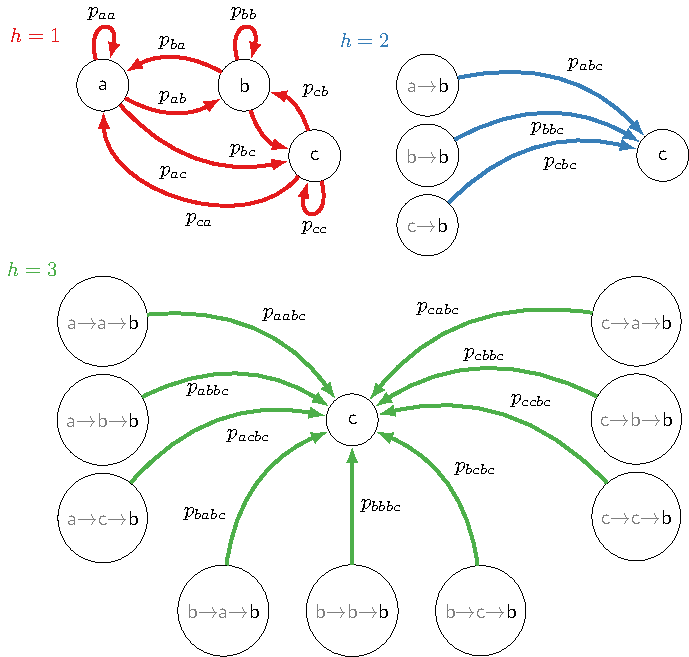
\includegraphics[width=\linewidth]{fig1a}
% \caption{\bf{Multi-step finite state Markovian processes}  parameterized by degree of memory $h$, demonstrated on a three-state network. For $h=1$, the statistics of the next state depend solely on the current state and the stochastic system is parameterized by transition probabilities indexed by a tuple. For $h=2$ and $h=3$ the statistics depend on the history.  Shown are the possible single-step transitions from state \bf{b} to state \bf{c}. For $h=2$, transition probabilities depend on the
% current state and the previous state, and all transition probabilities are indexed by $3$-tuples. For $h=3$, all transition probabilities depend on the current state and two previous states and are indexed by $4$-tuples. } \label{fig:fig1}
% \end{figure}
 
  \begin{figure}
 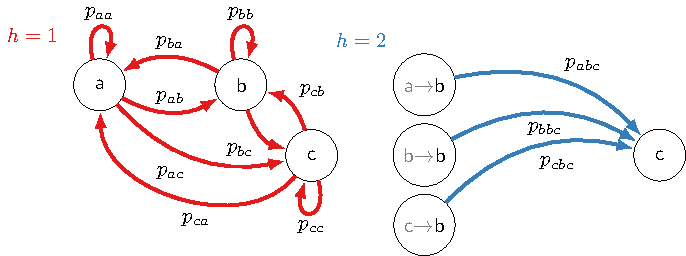
\includegraphics[width=\linewidth]{fig1b}
 \caption{\bf{Multi-step Markovian processes}  by degree of memory $h$, demonstrated on a three-state network. For $h=1$, the statistics of the next transition depend solely on the current state, and transition probabilities are indexed by  $2$-tuple. For $h\geq2$, the statistics depend on the history. For $h=2$, transition probabilities depend on the
 current state and the previous state, and all transition probabilities are indexed by $3$-tuples.  Shown are the possible single-step transitions from state \bf{b} to state \bf{c}.  } \label{fig:fig1}
 \end{figure}

There is a trade-off between complexity and fitting error that is inherent when varying $h$. From a statistical viewpoint, complexity results in less-precise determination of network parameters, leading to larger prediction errors. This undesirable consequence of complexity is known as \emph{overfitting}. Conversely, a simple model may not capture the true probability space where paths reside, and fail to catch patterns in the real process.

This Letter evaluates several statistical criteria for selecting the number of states worth of memory to retain in the factorization of Eq.~\ref{eq:factorize}, viewing the problem in terms of prediction accuracy. 
We wish to choose the value of $h$ that yields a model that best predicts new unobserved trajectories~\cite{claeskens2008model}. In particular, we seek to test the relationship between finding the best predictive model and uncovering the physical reality.

 For a fixed degree of memory $h$,
we may look at possible history vectors $\bx = [x_1,x_2,\ldots,x_h]$ of length $h$ taken from the set $\mathbf{X}_h = \{1,2,\ldots,M \}^h$. For each $\bx$, denote the vector $\mathbf{p}_{\bx} = [p_{\bx,1},p_{\bx,2},\ldots{p}_{\bx,M}],$ where $p_{\bx,m}$ is the probability that a trajectory goes next to state $m$ given that $\bx$ represents its most recent history. For convenience, we denote the collection of all $\bp_\bx$ as $\mathbf{p}$.  

Generally one has available some number of trajectories $J$. Assuming independence, one may write the joint probability, or likelihood, of observing these trajectories as
%\begin{align}
%\lefteqn{\Pr(\{\xi^{(j)} \}_{j=1}^J \vert \bp) = \prod_{j=1}^J \Pr(\xi^{(j)}\vert \bp)  } \nonumber\\
%&= \prod_{j=1}^J \prod_{\bx\in\mathbf{X}_h} \prod_{m=1}^M p_{\bx,m}^{N^{(j)}_{\bx,m}} = \prod_{\bx\in\mathbf{X}_h} \prod_{m=1}^M p_{\bx,m}^{N_{\bx,m}} ,
%\label{eq:likelihood}
%\end{align}
%\begin{align}
%\Pr(\{\xi^{(j)} \}_{j=1}^J \vert \bp) = \prod_{j=1}^J \Pr(\xi^{(j)}\vert \bp)  = \prod_{\bx\in\mathbf{X}_h} \prod_{m=1}^M p_{\bx,m}^{N_{\bx,m}} ,
%\label{eq:likelihood}
%\end{align}
%\begin{align}
\begin{align}
\Pr\left(\{\xi^{(j)} \}_{j=1}^J \vert \bp\right) = \smashoperator{\prod_{j=1}^J} \prod_{\bx\in\mathbf{X}_h} \prod_{m=1}^M p_{\bx,m}^{N^{(j)}_{\bx,m}} = \smashoperator{\prod_{\bx\in\mathbf{X}_h} }\ \prod_{m=1}^M p_{\bx,m}^{N_{\bx,m}} ,
\label{eq:likelihood}
\end{align}
where $N^{(j)}_{\bx,m}$ is the number of times that the transition $\bx\to m$ occurs in trajectory $\xi^{(j)}$, and $N_{\bx,m} = \sum_j N^{(j)}_{\bx,m}$ is the total number of times the transition is seen across all trajectories.% Eq.~\ref{eq:likelihood} can be found by grouping like terms of Eq.~\ref{eq:factorize}. 

For convenience,  denote $N_{\bx} =\sum_{m}N_{\bx,m}$,  $\bN_{\bx}= [\bN_{\bx,1},\bN_{\bx,2},\ldots,\bN_{\bx,M}]$, and the collection of all $\bN^{(j)}_{\bx}$ as $\bN$. The sufficient statistics of the likelihood are the counts, so we will refer to the likelihood as $\Pr(\bN\mid\bp)$. The maximum likelihood estimator for each parameter vector $\bp_\bx$ is found by maximizing the probability in Eq.~\ref{eq:likelihood}, and can be written easily as
$\hat{p}^{\textrm{MLE}}_{\bx} = \mathbf{N}_{\bx} / N_{\bx}$. 
Following this approach, the Akaike Information Criterion,~\cite{akaike1974new,tong1975determination,katz1981some}  %, $\textrm{AIC}=-2\log\Pr(\bN\vert \hat{p}^{\textrm{MLE}})+2k$,
which penalizes model complexity, may be used as a metric in order to choose a value of $h$.  Rooted in information theory, the AIC is an approximation of the information loss in the representation of data by a model~\cite{burnham2003model}. The model with the smallest AIC value, and hence with the smallest approximate loss, is chosen.

The aforementioned approach to the problem is simple, however, it has limitations. The AIC,  an asymptotic approximation of information loss, is not accurate for for small samples. A modification of the AIC known as the AICc exists~\cite{hurvich1989regression}, however, its exact form is problem specific~\cite{burnham2003model}. More fundamentally,
the maximum likelihood estimator precludes the existence of unobserved transitions -- a property that is problematic if  the sample size $J$ is small.
It is desirable to regularize the problem by allowing a nonzero probability that
transitions that have not yet been observed will occur. Our approach to rectifying these issues is Bayesian.

%Bayesian inference provides a natural way of instilling this property into the problem. Furthermore,
%after laying the Bayesian fundamentals, one has available a suite of theoretical tools. Most relevantly, Bayesian model comparison provides alternatives to the AIC that one may consider in finding the optimal degree of memory $h$. 

A natural Bayesian formulation of the
problem of determining the transition probabilities is to use the Dirichlet conjugate prior
on each parameter vector
$
\mathbf{p}_{\bx} \sim \mathrm{Dirichlet}(\boldsymbol\alpha),
$
 hyper-parameterized by $\boldsymbol\alpha$, a vector of size $M$. This Letter assumes that $\alpha=\mathbf{1}$, corresponding to a uniform prior. This prior, paired with the likelihood of Eq.~\ref{eq:likelihood}, %yields the posterior distribution on the probabilities,
%\begin{equation}
%\mathbf{p}_{\bx}  \vert \mathbf{N}_{\bx} \sim \mathrm{Dirichlet}(\boldsymbol\alpha + \mathbf{N}_{\bx} ).
%\label{eq:posterior}
%\end{equation}
%According to this distribution, the posterior expectations for the transition probabilities follow
%\begin{equation}
%\mathbb{E}_{\bp_\bx\vert\bN_\bx} [p_{\bx,m}] = \frac{\alpha + N_{\bx,m}}{M\alpha+ N_{\bx}}.
%\end{equation}
yields the a posterior Dirichlet distribution with associated expectation,
\begin{equation}
\mathbf{p}_{\bx}  \vert \mathbf{N}_{\bx} \sim \mathrm{Dirichlet}(\boldsymbol\alpha + \mathbf{N}_{\bx} ) \quad \mathbb{E}_{\bp_\bx\vert\bN_\bx} [p_{\bx,m}] = \frac{\alpha + N_{\bx,m}}{M\alpha+ N_{\bx}}.\label{eq:posterior}
\end{equation}
In effect, one is assigning a probability of $\alpha/(M\alpha+N_{\bx})$ to any unobserved transition, where $\alpha$ can be made small if it is expected that the transition matrix should be sparse.   In the asymptotic limit, the choice of $\alpha$ is not important as the posterior distribution of Eq.~\ref{eq:posterior}  becomes tightly concentrated about the maximum likelihood estimates.

As pertains to Bayesian model selection,  Bayes factors are often used~\cite{lavine1999bayes,posada2004model}. If using non-informative model priors, they consist of the likelihood of the data, averaged over the posterior distribution of model parameters. The logarithm of this quantity is known as the log predictive density (LPD). Related to the LPD is the log pointwise predictive density (LPPD), where the same expectation is taken separately for each datapoint and logarithms of these expectations are summed. The LPPD features in alternatives to Bayes factors and the AIC~\cite{gelman2014understanding}.

The Widely Applicable Information Criterion~\cite{watanabe2010asymptotic,watanabe2013widely} (WAIC) is a Bayesian information criterion that consists of two variants, WAIC$_1$, and WAIC$_2$, each featuring the LPPD but differing in how they compute model complexity.  The WAIC, unlike the AIC, is applicable to singular statistical models and is asymptotically equivalent to Bayesian cross-validation~\cite{watanabe2010asymptotic}. The commonly used Deviance Information Criterion (DIC) also resembles the WAIC,  consisting of two variants DIC$_1$ and DIC$_2$. Both variants of the DIC use point estimates of the posterior parameters rather than expectations as used in the WAIC.
However, unlike the WAIC and cross-valdation, Bayes factors, DIC, and other methods using the BIC~\cite{narlikar2013one} do not have as their objective the maximization of predictive model fit onto new data~\cite{gelman2014understanding}.

Finally Bayesian variants of cross-validation have recently been proposed as alternatives to information criterion~\cite{gelman2014understanding}. It is of note that the WAIC provides an asymptotic approximation of cross-validation (CV). In our problem, $k$-fold CV, where data is divided into $k$ partitions, can be evaluated in closed form without repeated model fitting. Using $-2\times \textrm{LPPD}$ as a metric, this Letter also evaluates two variants of $k$-fold CV:
two-fold cross validation (LPPDCV$_2$) and leave-one-out cross validation (LOO).
  %%%%%%%%%%%%%%%%%%%

\begin{figure*}[!ht]
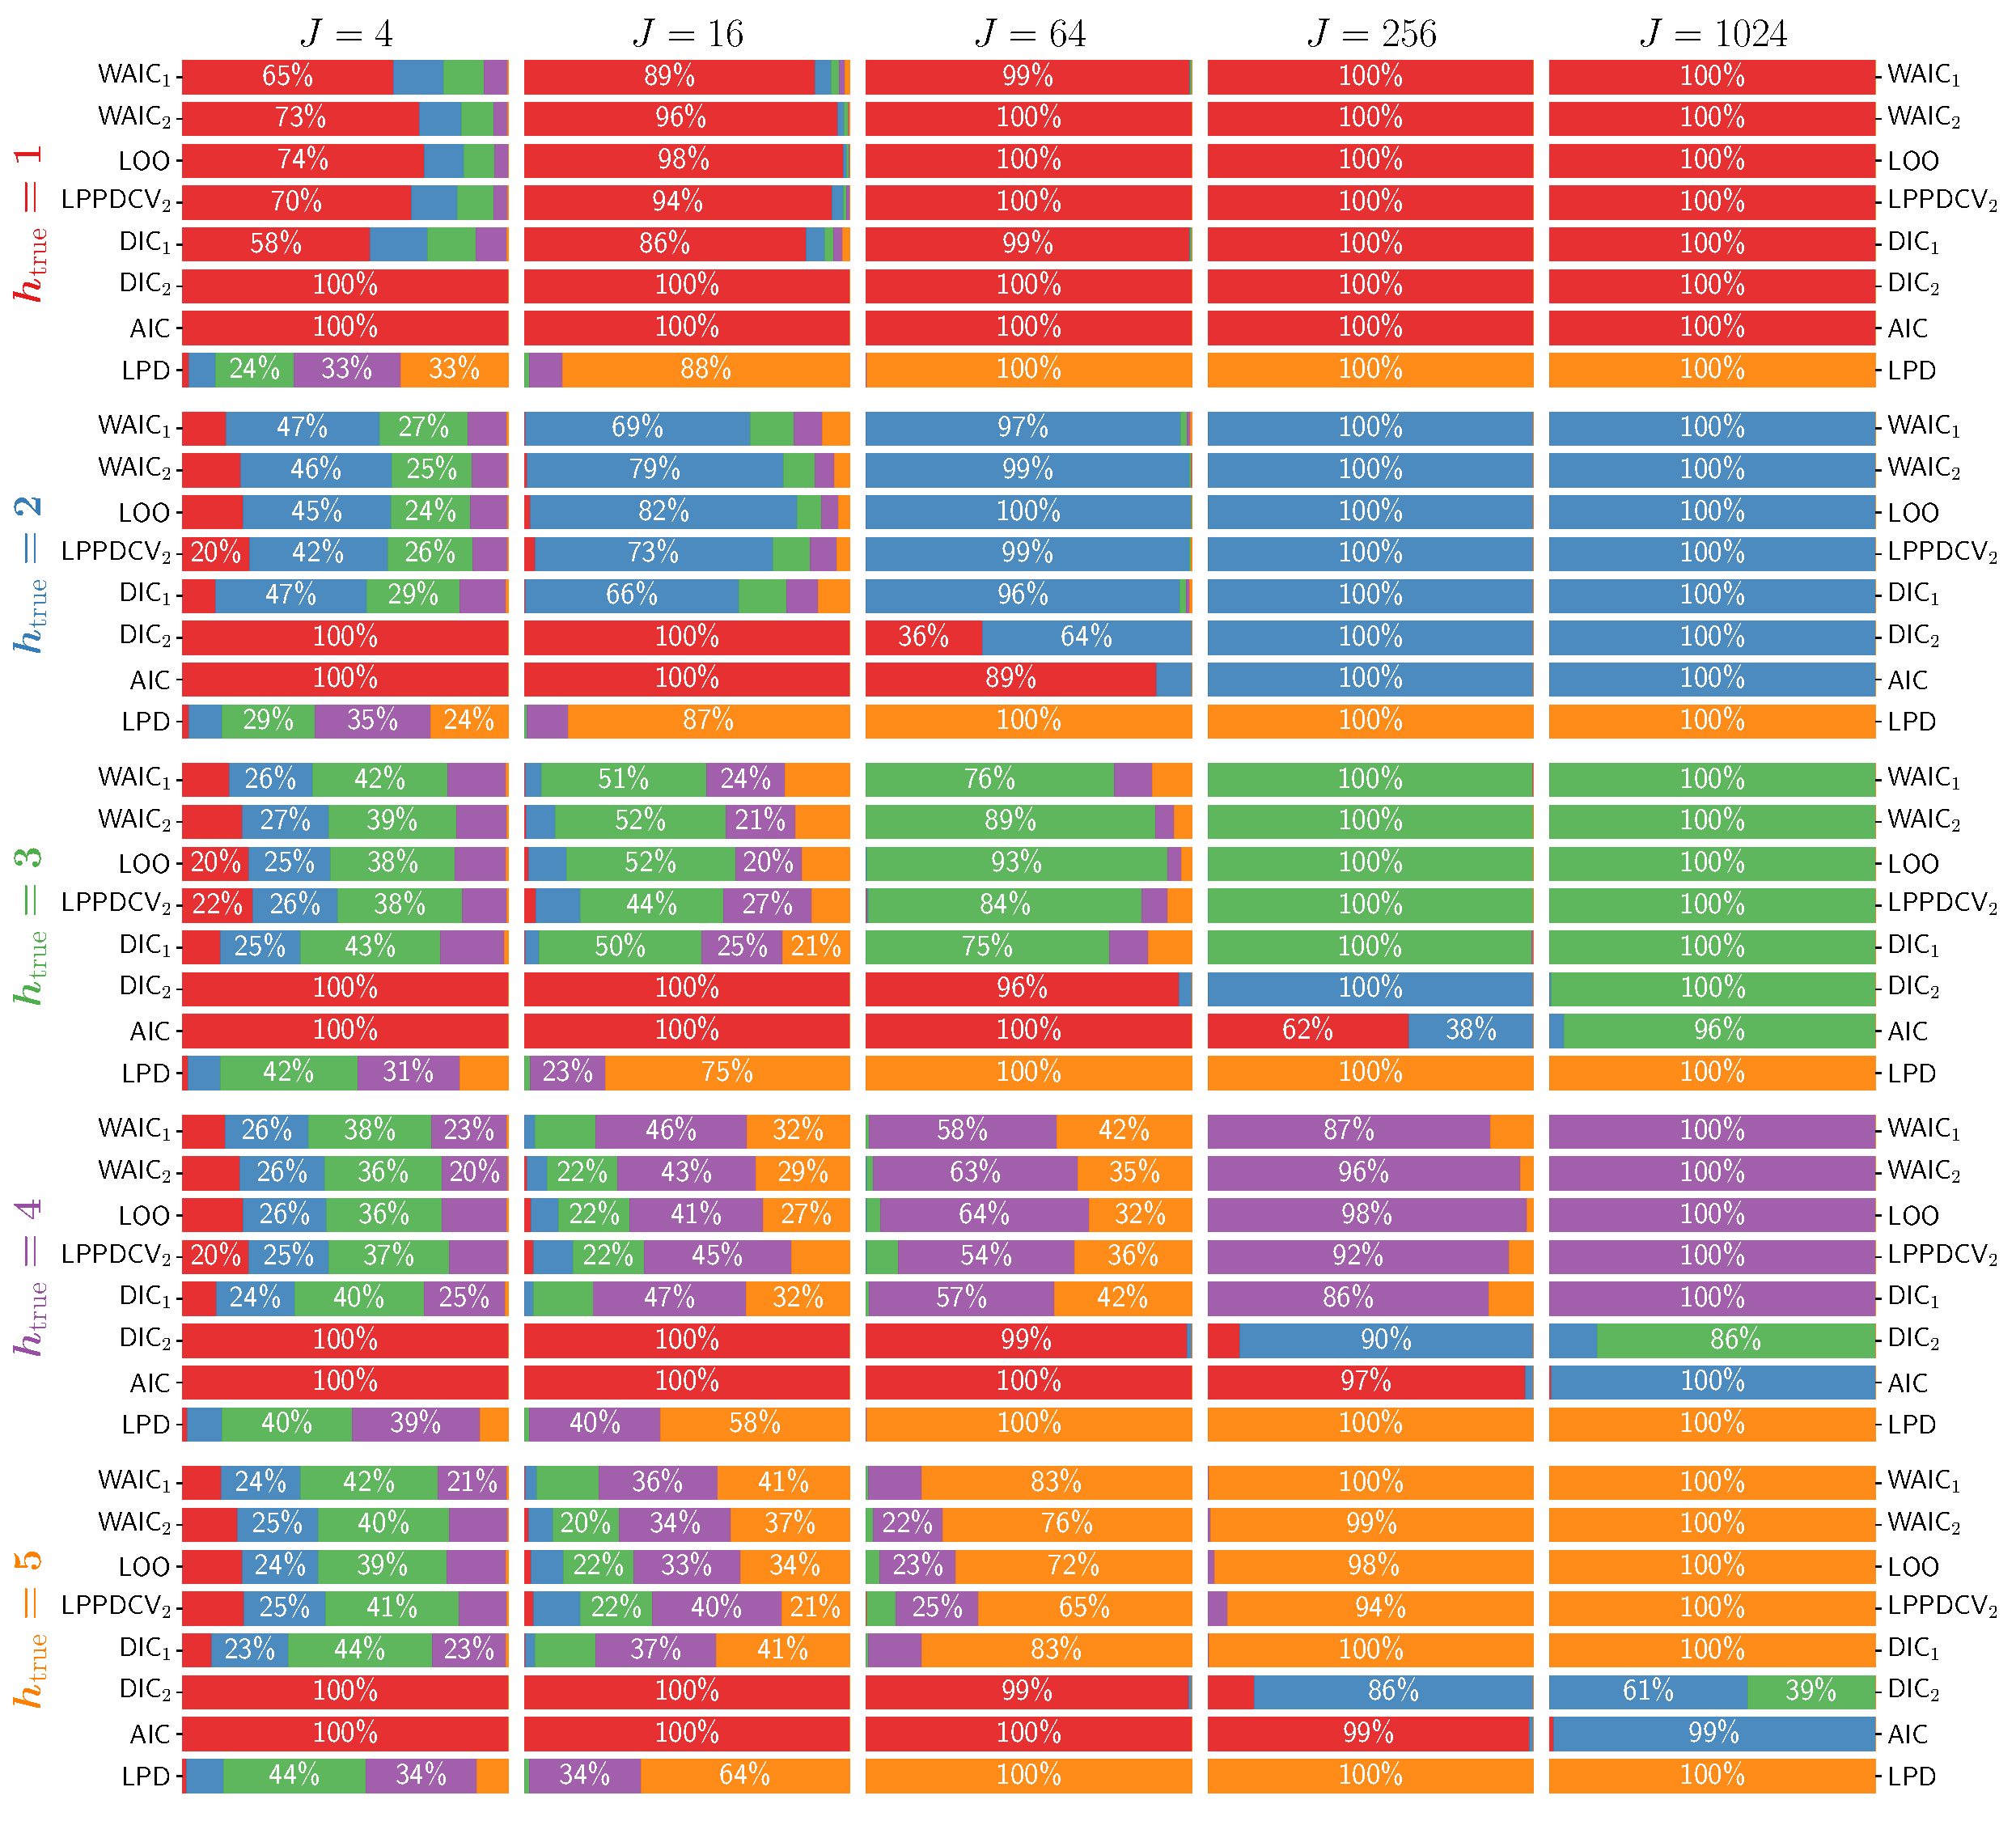
\includegraphics[width=\textwidth]{fig2}
\caption{\textbf{Chosen degree of memory $h$} in simulations for varying true degrees of memory  $h_{\textrm{true}}$ and number of observed trajectories $J$. Rows correspond to model selection under a given degree of memory. Columns correspond to the number of trajectories. Depicted are the percent of simulations in which each degree of memory is selected using the different model evaluation criteria (percents of at least $20$ are labeled). Colors coded based on degree of memory: ({\color{Set1_5_red} 1: red}, {\color{Set1_5_blue} 2: blue}, {\color{Set1_5_green}3: green}, {\color{Set1_5_purple}4: purple}, {\color{Set1_5_orange}5: orange}). \emph{Example:} For $h_{\textrm{true}}=1$ and $J=4$, the WAIC$_1$ criteria selected $h=1$ approximately $65\%$ of the time. }
\label{fig:fig2}
\end{figure*}


To e these methods, we evaluated them  using simulations. Closed-form formulae for computing each model selection criterion are available as \textsc{Supplemental material}. Our test system is composed of $M=8$ states, with designated start and absorbing states.  For each given value of $h$, we generated for each $\bx\in \mathbf{X}_h$ a single set of true transition probabilities drawn from Dirichlet($\mathbf{1}$) distributions. For each of these random networks of a fixed $h$, we randomly sampled trajectories of a given sample size $J$ $10^4$ times, determining from each sample of $J$ the degree of $h$ to use as chosen by each of the methods.

\begin{figure}
\includegraphics[width=\linewidth]{fig3}
\caption{\textbf{Distributions of computed selection criteria relative to a true model ($h_{\textrm{true}}=2$)}, $\Delta\textrm{Criterion}(h)=\textrm{Criterion}(h)-\textrm{Criterion}(h_{\textrm{true}})$.  Density plots with minimum, maximum, and mean of the selection criteria for each model relative to that of the true model are shown at various sample sizes $J$. Values above zero mean that the true model is favored over a particular model. Ideally, mass should be above zero for accurate selection of the true model (zero drawn as dashed line).}
\label{fig:fig3}
\end{figure}

Fig.~\ref{fig:fig2} provides the frequency that each of five models ($h=1,\ldots,5$) was chosen based on the selection criteria compared. Each row corresponds to a given true degree of memory $h_{\textrm{true}}$ and the columns represent increasing sample sizes when viewed from left to right. Generally, it is seen that as the number of samples increases, all selection criteria except for the LPD (Bayes factors) improve in their ability to select the true model.  In general, the AIC does well if the true memory is small, but requires more data than many of the competing methods in order to resolve larger degrees of memory. 

The two variants of the WAIC, LOO, and DIC$_1$ perform roughly on par. Since each criterion selects the model with the lowest value, it is desirable that $\Delta\textrm{Criterion}(h)=\textrm{Criterion}(h)-\textrm{Criterion}(h_{\textrm{true}})>0$, for $h\neq h_{\textrm{true}}$. Fig.~\ref{fig:fig3} explores the distributions of these quantities in the case where $h_{\textrm{true}}=2$.  As sample size $J$ increases, there is clearer separation of the masses of these quantities from zero. By $J=64$, for instance, no models where $h=1$ are selected using any of the criteria. The WAIC$_2$ and LOO criteria perform about the same whereas the WAIC$_1$ criteria and the DIC$_1$ criteria lag behind in separating themselves from zero.


As a result of these tests, this Letter recommends the leave-one-out cross validation criterion:
\begin{equation}
\textrm{LOO} = -2\sum_j \sum_{\bx}  \log\left(  \frac{B(\bN_\bx  +\balpha)}{B(\bN_\bx -\bN_{\bx}^{(j)} +\balpha)} \right),
\label{eq:loo}
\end{equation}
where $B$ is the multivariate Beta function. LOO performed slightly better than WAIC$_2$ in the included tests, while being somewhat simpler to compute. Eq.~\ref{eq:loo} decomposes completely into a sum of logarithms of Gamma functions, and is hence easy to implement in standard scientific software packages.

A simple real-world application of this method is the evaluation of ``hot-hand phenomenon'' (or fallacy) in the context of basketball free-throw shooting. This phenomenon is controversial. In 1985, 

  During the 2016-2017 season, through $100$ games, LeBron James of the Cleveland Cavaliers attempted $693$ total free throws, hitting $471$ of them for $68.0\%$ accuracy.

This Letter has shown that LOO and WAIC$_2$ can learn from data the physical reality of the 
degree of memory in a system. It is important to comment on the uncertainty in such determinations. Regardless of the selection criterion used, the determination of $h$ is not truly certain except in an asymptotic sense where one has an unlimited amount of data available. However, one may use a simulation procedure like the one used in this Letter in order to estimate the degree of uncertainty.  

Importantly,   both the AIC and LPD (Bayes factors) are biased, in opposite directions. The AIC tends to sparsity, which runs counter to the typical situation in linear regression problems where the AIC can favor complexity with too few data, a situation ameliorated by the more-stringent AICc~\cite{claeskens2008model}. Bayes factors with flat model  priors as investigated here, on the other hand, are known to automatically penalize complexity indirectly through increased posterior entropy. Yet, when enough data are present, posterior entropy is low while many model parameters may be highly concentrated about zero and the Bayes factor is happy to select the more-complex model even if it is inconsistent with physical truth.
%
Notably, alternative Bayes factors methods for selecting the degree of memory also include model-level priors that behave like the penalty term in the AIC~\cite{strelioff2007inferring,singer2014detecting}. Since the upper bound of the LPD is the logarithm of the likelihood found from the MLE procedure, this selection method is more stringent in the low sample-size regime than the pure AIC and hence will suffer from the same bias towards less memory.


Models of structure similar to Eq.~\ref{eq:factorize} have appeared in limitless contexts such as in text analysis~\cite{melnyk2006memory}, analysis of human digital trails~\cite{singer2014detecting}, DNA sequence analysis, protein folding~\cite{yuan1999prediction}, and biology~\cite{bettenbuhl2012bayesian}. As we have seen, many methods tend to asymptotically select the correct model. However, studies are seldom in the asymptotic regime and the use of the methods mentioned in this Letter to reanalyze data from prior studies may prove fruitful in uncovering previously overlooked physics. The general method mentioned in this Letter can also be extended to model averaging in order to generate jagged models with no single fixed degree of memory.





\emph{Acknowledgements} The author thanks the United States Social Security Administration and the Intramural Research Program at the NIH Clinical Center for funding this research. Additionally, the author is thankful for helpful comments from members of the Biostatistics and Rehabilitation Section in the Rehabilitation Medicine Department at NIH, John P. Collins in particular, and also Carson Chow at NIDDK.

\bibliographystyle{plain}
\bibliography{markovpaths}

%%%%%%%%%%%%%%%%%%%%%%%%%%%%%%%%%%%
\clearpage
\newpage
\appendix

\section{Supplemental Material: Computation of alternate model validation criteria}


The Akaike information criterion (AIC) is defined through the formula $\textrm{AIC}  = -2 \sum_{\bx}\log \Pr(\bN_\bx \vert \hat{\bp}_{\textrm{MLE}}) + 2k$ and can be computed exactly as
\begin{align}
\textrm{AIC}  &= -2\sum_{\bx}\sum_{m=1}^M N_{\bx,m}\log \left( \frac{N_{\bx,m}}{N_\bx} \right)+ 2M^{q+1},
\end{align}
where we define $0\times\log(0)=0$.


 The deviance information criterion (DIC) is similar to the AIC and defined as 
$\textrm{DIC} = -2\sum_{\bx}\log p\left(\bN_{\bx} \mid \bp_{\bx} = \mathbb{E}_{\bp_{\bx}\vert \bN_\bx}  \bp_{\bx}   \right) + 2k_{\textrm{DIC}}.$ It may also be computed by evaluating the closed form expression
\begin{equation}
\textrm{DIC} =-2\sum_{\bx}\sum_{m=1}^M N_{\bx,m}\log \left( \frac{N_{\bx,m} +\alpha}{N_\bx+ M\alpha}  \right)+  2k_{\textrm{DIC}},
\end{equation}
where we are assuming that one uses the posterior mean as the point estimate of the model parameters, and also where the effective model complexity $k_{DIC}$ has two variants
 \begin{align}
\lefteqn{ k_{\textrm{DIC1}}= -2\Bigg\{ \sum_{\bx}\sum_{m=1}^M N_{\bx,m}\log \left( \frac{N_{\bx,m} +\alpha}{N_\bx+ M\alpha}  \right)   } \nonumber\\
 & -\sum_j \sum_\bx \mathbb{E}_{\bp_\bx\vert\bN}\log\bp_\bx^{\bN_{\bx}^{(j)}} \Bigg\} \nonumber\\
 &=2\Bigg\{ \sum_{\bx}\sum_{m=1}^M N_{\bx,m}\log \left( \frac{N_{\bx,m} +\alpha}{N_\bx+ M\alpha}  \right)   \nonumber\\
 & -\sum_j \sum_\bx \sum_{m=1}^M {\bN_{\bx,m}^{(j)}}  \left[ \psi(\alpha+N_{\bx,m}) - \psi(M\alpha+N_{\bx}) \right] \Bigg\} \nonumber\\
  &=2\Bigg\{ \sum_{\bx}\sum_{m=1}^M N_{\bx,m}\log \left( \frac{N_{\bx,m} +\alpha}{N_\bx+ M\alpha}  \right)   \nonumber\\
 & - \sum_\bx \sum_{m=1}^M {N_{\bx,m} }  \left[ \psi(\alpha+N_{\bx,m}) - \psi(M\alpha+N_{\bx}) \right] \Bigg\} ,\nonumber\\
  \end{align}
  %
  and $k_{\textrm{DIC2}} = 2\textrm{var}_{\bp\mid\bN}\left[ \log \Pr\left( \bN\mid \bp\right) \right] ,$ which may be computed
  %
 \begin{align}
\lefteqn{k_{\textrm{DIC2}} =2 \var_{\bp_\bx}\left[ \sum_{\bx}\sum_{m} N_{\bx,m} \log p_{\bx,m}  \right] }\nonumber \\
&=2\sum_{\bx} \var_{\bp_\bx}\left( \sum_{m} N_{\bx,m} \log p_{\bx,m} \right) \nonumber\\
&=2\sum_{\bx} \sum_{m}\sum_{n} N_{x,m}N_{x,n} \cov(\log p_{\bx,m},\log p_{\bx,n}) \nonumber\\
&=2\sum_{\bx} \sum_m\sum_n N_{x,m}N_{x,n} \nonumber\\
&\qquad\qquad\qquad\times\left[ \psi^\prime(\alpha+N_{\bx,m})\delta_{mn} - \psi^\prime(M\alpha+N_{\bx})  \right] \nonumber\\
&=2\sum_{\bx} \left(\sum_m N_{\bx,m}^2 \psi^\prime(\alpha+N_{\bx,m})  - (N_{\bx})^2  \psi^\prime(M\alpha+N_{\bx}) \right)
\end{align}
Bayes factors are ratios of the probability of the dataset given two models and their corresponding posterior parameter distributions. In the case of this application, the likelihood completely factorizes into  a product of transition probabilities and each model's corresponding term in a Bayes factor is the exponential of its log predictive density (LPD). The LPD can be computed exactly
\begin{align}
\lefteqn{\textrm{LPD} = \log\mathbb{E}_{\bp\vert\bN}  \left[     \Pr\left(\mathbf{N}  \mid \bp \right) \right] } \nonumber\\
&=  \log \mathbb{E}_{\bp\vert\bN} \left( \prod_\bx  \prod_{m=1}^{M} p_{\bx,m}^{N_{\bx,m}} \right) \nonumber \\
&= \sum_{\bx} \log\left( \frac{B(2\bN_\bx+\balpha)}{B(\bN_\bx +\balpha )} \right).
\end{align}

Related to the LPD is the log pointwise predictive density (LPPD), where the expectation in
the LPD is broken down ``point-wise.'' For our application, we will consider trajectories to be
points and write the LPPD as
\begin{align}
\lefteqn{\textrm{LPPD} = \sum_j\sum_{\bx}\log\mathbb{E}_{\bp_\bx\vert\bN_\bx}  \left[     \Pr\left(\mathbf{N}^{(j)}_{\bx} \mid \bp_\bx \right) \right] } \nonumber\\
&= \sum_j\sum_{\mathbf{x}} \log \mathbb{E}_{\bp_\bx\vert\bN_\bx} \left(% \frac{N_{\mathbf{x}}!}{\mathbf{N}_{\mathbf{x}}!}  
 \prod_{m=1}^{M} p_{\bx,m}^{N^{(j)}_{\bx,m}} \right) \nonumber\\
&=\sum_j \sum_{\bx}  \log\left(  \frac{B(\bN_\bx +\bN_{\bx}^{(j)} +\balpha)}{B(\bN_\bx +\balpha)} \right).
\end{align}

The WAIC is defined as $\textrm{WAIC} = -2\textrm{LPPD}+2k_{\textrm{WAIC}}$, where the effective model sizes are computed exactly as
\begin{align}
\lefteqn{k_{\textrm{WAIC1}} = 2\textrm{LPPD}-2\sum_j \sum_\bx \mathbb{E}_{\bp_\bx\vert\bN}\log\bp_\bx^{\bN_{\bx}^{(j)}}  }\nonumber \\
&= 2 \textrm{LPPD} -  \sum_j\sum_{\bx}\sum_{m=1}^M N_{\bx,m}^{(j)} \mathbb{E}_{\bp_\bx\vert \bN_\bx} \left(\log p_{\bx,m} \right) \nonumber\\
& = 2 \textrm{LPPD} \nonumber\\
&\quad- 2\sum_j \sum_\bx  \sum_{m=1}^MN_{\bx,m}^{(j)} \left[ \psi(N_{\bx,m}+ \alpha ) - \psi(N_{\bx}  + M\alpha ) \right]  \nonumber\\
&= 2 \textrm{LPPD} \nonumber\\
&\quad- 2\sum_{\bx}\sum_{m=1}^M N_{\bx,m}\left[ \psi(N_{\bx,m}+ \alpha ) - \psi(N_{\bx}  + M\alpha ) \right],
\end{align}
and
\begin{align}
\lefteqn{k_{\textrm{WAIC2}} =\sum_j \sum_\bx \var_{\bp_\bx}\left[ \log  \Pr\left(\mathbf{N}^{(j)}_{\bx} \mid \bp_\bx \right)   \right] }\nonumber \\
&=\sum_j\sum_{\bx} \var_{\bp_\bx}\Bigg\{ \log\left( %\frac{N_{\mathbf{x}}!}{\mathbf{N}_{\mathbf{x}}!}  
\prod_{m=1}^{M} p_{\bx,m}^{N^{(j)}_{\bx,m}} \right)   \Bigg\} \nonumber\\
&=\sum_j\sum_\bx   \var_{\bp_\bx}\left[  \sum_{m=1}^M N^{(j)}_{\bx,m} \log p_{\bx,m} \right] \nonumber\\
&= \sum_j\sum_\bx \sum_{m=1}^M \sum_{n=1}^M N^{(j)}_{\bx,m} N^{(j)}_{\bx,n} \cov\left( \log p_{\bx,m}, \log p_{\bx,n} \right) \nonumber\\
&= \sum_j\sum_\bx \sum_{m=1}^M \sum_{n=1}^M N^{(j)}_{\bx,m} N^{(j)}_{\bx,n}\Bigg[  \psi^\prime\left( \alpha+N_{\bx,n} \right)\delta_{nm} \nonumber\\
&\qquad\qquad\qquad- \psi^\prime\left( M\alpha+N_\bx \right) \Bigg] \nonumber\\
&=\sum_j \sum_\bx \Bigg[\sum_{m=1}^M [N^{(j)}_{\bx,m}]^2\psi^\prime(\alpha+N_{\bx,m}) \nonumber\\
&\qquad\qquad\qquad-[N^{(j)}_{\bx}]^2\psi^\prime(M\alpha+N_\bx)  \Bigg].
\end{align}
Finally, as an alternative to information criterion, we may use cross-validation. In particular, the log posterior predictive density under leave-one-out cross validation (LOO)
has a particularly simple form,
\begin{equation}
\textrm{LOO} = -2\sum_j \sum_{\bx}  \log\left(  \frac{B(\bN_\bx  +\balpha)}{B(\bN_\bx -\bN_{\bx}^{(j)} +\balpha)} \right) .
\end{equation}
The leave-one-out version of cross validation is a specific case of $k$-fold cross validation, where $k$ is precisely the number of data points. At the other extreme of this type of cross validation is $2$-fold cross validation, which can be computed exactly as
\begin{align}
\textrm{LPPD}\textrm{CV}_2 &= -2\sum_{j=1}^{J/2} \sum_{\bx}  \log\left(  \frac{B(\bN^+_\bx +\bN_{\bx}^{(j)} +\balpha)}{B(\bN^+_\bx+\balpha)} \right)  \nonumber\\
& -2 \sum_{j=J/2}^{J} \sum_{\bx} \log\left(  \frac{B( \bN^-_\bx +\bN_{\bx}^{(j)} +\balpha)}{B( \bN^-_\bx +\balpha)} \right),
\end{align}
where $\bN^\pm_\bx$ constitute the transition counts of the last $J/2$ trajectories or the first $J/2$ trajectories respectively, so that $\bN^-_\bx + \bN^+_\bx = \bN_\bx$.

\end{document}  